\documentclass[UTF8]{article}

\usepackage{amsmath, amsfonts, amssymb, amstext, amscd, amsthm, bbm, CJKutf8, color, dsfont, enumerate, float, graphicx, hyperref, makeidx, mathrsfs, mathtools, marvosym, soul, url, verbatim, xcolor, xfrac}
\usepackage[left=2cm,top=2cm,right=2cm,bottom=2cm,bindingoffset=0cm]{geometry}
\allowdisplaybreaks 
\newenvironment{subproof}[1][Proof]
    {\proof[#1]\leftskip=1cm\rightskip=1cm}
	{\endproof}

%theorems with custom numbering
%\newtheorem{innerthm}{Theorem}
%\newenvironment{thm}[1]
    %{\renewcommand\theinnerthm{#1}\innercustomthm}
    %{\endinnerthm}

\newtheorem{theorem}{Theorem}
\newtheorem{lemma}{Lemma}
\newtheorem{proposition}{Proposition}
\newtheorem{corollary}{Corollary}
\newtheorem{claim}{Claim}
\newtheorem{conjecture}{Conjecture}
\newtheorem{justification}{Justification}
\newtheorem{definition}{Definition}
\newtheorem*{remark}{Remark}
\newtheorem*{note}{Note}

\renewcommand{\and}{\;\wedge\;}
\newcommand{\disj}{\;\vee\;}
\newcommand{\xor}{\;\oplus\;}
\newcommand{\divides}{\;|\;}
\newcommand{\suchthat}{\;\middle|\;}
\newcommand{\contradiction}{\;\text{\Large \Lightning}}
\newcommand{\conj}[1]{\overline{#1}}
\newcommand{\mean}[1]{\overline{#1}}
\newcommand{\integral}[1]{\smashoperator{\int_{#1}}}
\renewcommand{\restriction}[1]{\downharpoonright_{#1}}
\renewcommand{\qedsymbol}{QED} 
\DeclareMathOperator{\lcm}{lcm}
\DeclareMathOperator*{\argmin}{arg\!\min}
\DeclareMathOperator*{\argmax}{arg\!\max}

\let\originalleft\left
\let\originalright\right
\renewcommand{\left}{\mathopen{}\mathclose\bgroup\originalleft}
\renewcommand{\right}{\aftergroup\egroup\originalright}
\newcommand{\zh}[1]{\begin{CJK}{UTF8}{gbsn}#1\end{CJK}}
\newcommand{\jp}[1]{\begin{CJK}{UTF8}{gbsn}#1\end{CJK}}

\DeclarePairedDelimiterX \inner[2]{\langle}{\rangle}{#1,#2}
\DeclarePairedDelimiterX \braket[2]{\langle}{\rangle}{#1 \delimsize\vert #2}
\DeclarePairedDelimiter \bra{\langle}{\rvert}
\DeclarePairedDelimiter \ket{\lvert}{\rangle}
\DeclarePairedDelimiter \abs{\lvert}{\rvert}
\DeclarePairedDelimiter \lrangle{\langle}{\rangle}
\DeclarePairedDelimiter \norm{\lVert}{\rVert}
\DeclarePairedDelimiter \set{\lbrace}{\rbrace}
\DeclarePairedDelimiter \parens{(}{)}

\begin{document}
\begin{center}
	\textsc{\huge Applied Machine Learning}\\
	\textsc{\Large Homework 10}\\
\end{center}
\begin{flushright}
	Daniel Gonzalez\\
    Colton Piper\\
	$15^{\text{th}}$ of November, $2018$
\end{flushright}


\section{Results}
For this assignment, we used the \texttt{GaussianMixture} package from SciKitLearn for Python to call the EM algorithm.

\subsection{Table}

\begin{table}[H]
\centering
    \caption{One-Step EM Algorithm}
    \begin{tabular}{|l|l|l|l|l|}
        \hline
        Data Set & $k$ & $\pi_k$ & $\mu_k$ & $\Sigma_k$\\\hline

        \texttt{xeasy}  & 1 & $0.407871$    & $(0.02478088, 3.07460079)$    & \begin{pmatrix} 1.01363993 & -0.05311694 \\ -0.05311694   & 0.94863522\end{pmatrix}\\\cline{2-5}
                        & 2 & $0.592129$    & $(3.01650103, -0.17460086)$   & \begin{pmatrix} 1.00808335 & 0.15670429 \\ 0.15670429     & 0.94521241\end{pmatrix}\\\hline

        \texttt{x1} & 1 & $0.55565978$  & $(-0.28366821, 2.16960597)$   & \begin{pmatrix} 1.59256984    & 0.35809924 \\ 0.35809924      & 2.07505554\end{pmatrix}\\\cline{2-5}
                    & 2 & $0.44434022$  & $(1.83617659, 0.28263171)$    & \begin{pmatrix} 1.12412731    & -0.09771768 \\ -0.09771768    & 1.22889663\end{pmatrix}\\\hline

        \texttt{x2} & 1 & $0.56150159$  & $(0.03484, -0.03989854)$      & \begin{pmatrix} 1.31365667 & 0.10374308 \\ 0.10374308 & 0.97577869\end{pmatrix}\\\cline{2-5}
                    & 2 & $0.43849841$  & $(0.17023148, -0.14255449)$   & \begin{pmatrix} 9.86732223 & 0.79962458 \\ 0.79962458 & 10.26300564\end{pmatrix}\\\hline
\end{tabular}
\end{table}

\begin{table}[H]
\centering
    \caption{Two-Step (Provable) EM Algorithm}
    \begin{tabular}{|l|l|l|l|l|}
        \hline
        Data Set & $k$ & $\pi_k$ & $\mu_k$ & $\Sigma_k$\\\hline

        \texttt{xeasy}  & 1 & $0.59388969$    & $(3.01183881, -0.17000872)$ & \begin{pmatrix} 1.01430655 & 0.14999363 \\ 0.14999363 & 0.95097821\end{pmatrix}\\\cline{2-5}
                        & 2 & $0.40611031$    & $(0.01862825, 3.08197222)$  & \begin{pmatrix} 1.00648418 & -0.0442361 \\ -0.0442361 & 0.93800178\end{pmatrix}\\\hline

        \texttt{x1} & 1 & $0.74863867$  & $(1.08395907, 0.85578155)$    & \begin{pmatrix} 2.1600946 & -0.51568872 \\ -0.51568872 & 1.99120546\end{pmatrix}\\\cline{2-5}
                    & 2 & $0.25136133$  & $(-0.6095988, 2.74694693)$    & \begin{pmatrix} 1.34102811 & 0.62338099 \\ 0.62338099 & 1.64899629\end{pmatrix}\\\hline

        \texttt{x2} & 1 & $0.54930196$  & $(0.03588655, -0.03956158)$   & \begin{pmatrix} 1.28017758 & 0.10341123 \\ 0.10341123 & 0.94265068\end{pmatrix}\\\cline{2-5}
                    & 2 & $0.45069804$  & $(0.16529115, -0.14018644)$   & \begin{pmatrix} 9.67740853 & 0.78075241 \\ 0.78075241 & 10.05218714\end{pmatrix}\\\hline
\end{tabular}
\end{table}

\section{Figures}
\begin{figure}[H]
    \centering
    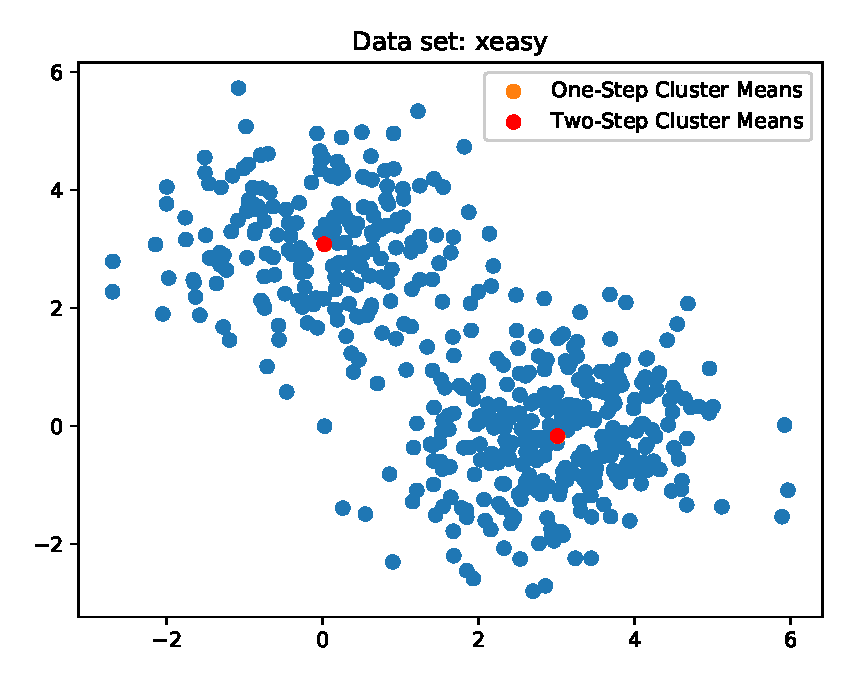
\includegraphics[scale=0.95]{./figures/xeasy.eps}
\end{figure}
\begin{figure}[H]
    \centering
    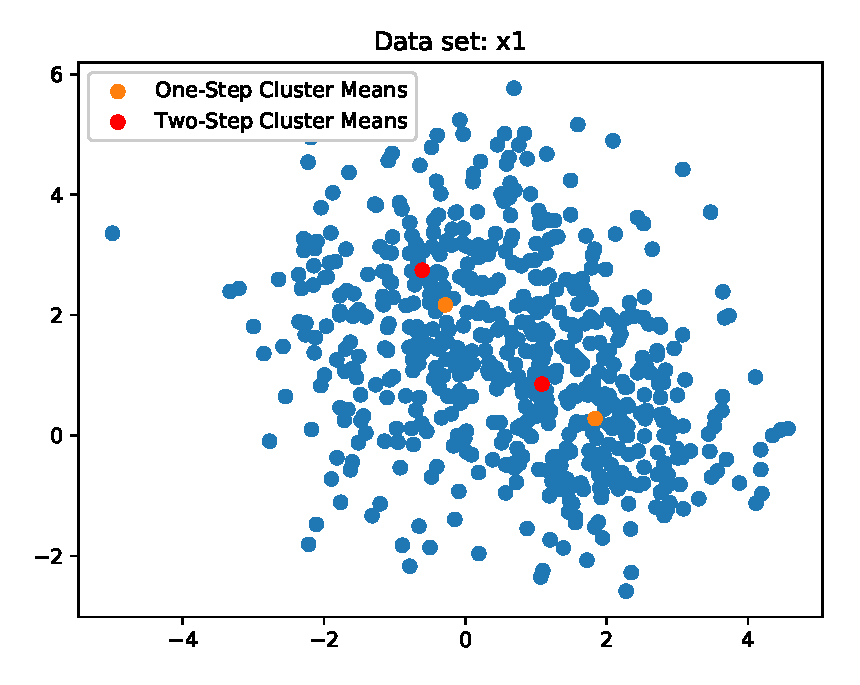
\includegraphics[scale=0.95]{./figures/x1.eps}
\end{figure}
\begin{figure}[H]
    \centering
    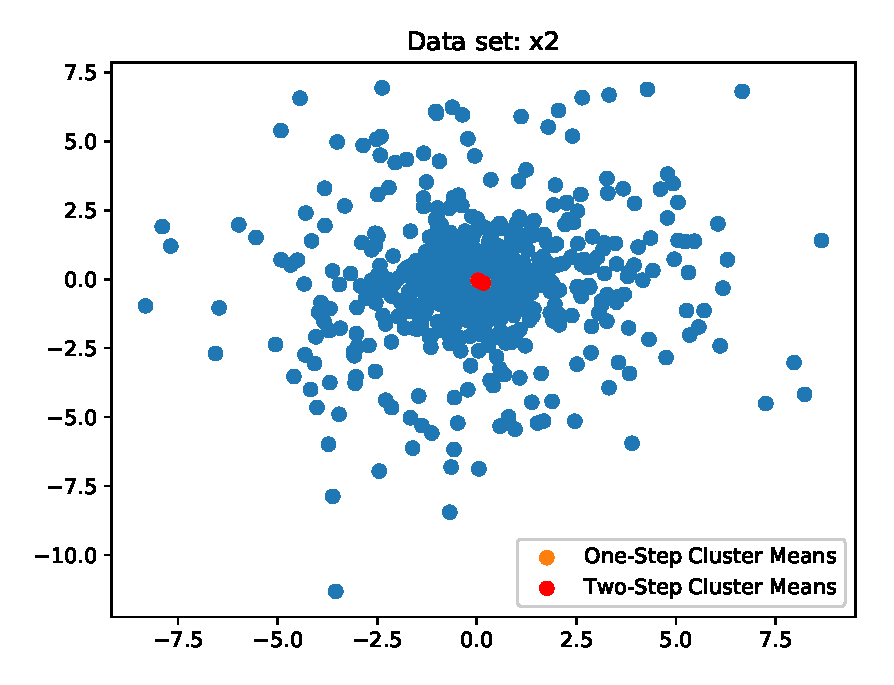
\includegraphics[scale=1.2]{./figures/x2.eps}
\end{figure}

\section{Appendix: Code}
If the code looks too small, please zoom in on the pdf.
The screenshots are \texttt{.png} images, so you should be able to zoom in and read at whatever is a comfortable size for you.
The first two screenshots are of the actual EM code, while the last screenshot is the python code for graphing to verify our results.
\begin{figure}[H]
    \centering
    \includegraphics[scale=0.85]{./figures/narrowcode1.png}
\end{figure}
\begin{figure}[H]
    \centering
    \includegraphics[scale=0.85]{./figures/narrowcode2.png}
\end{figure}
\begin{figure}[H]
    \centering
    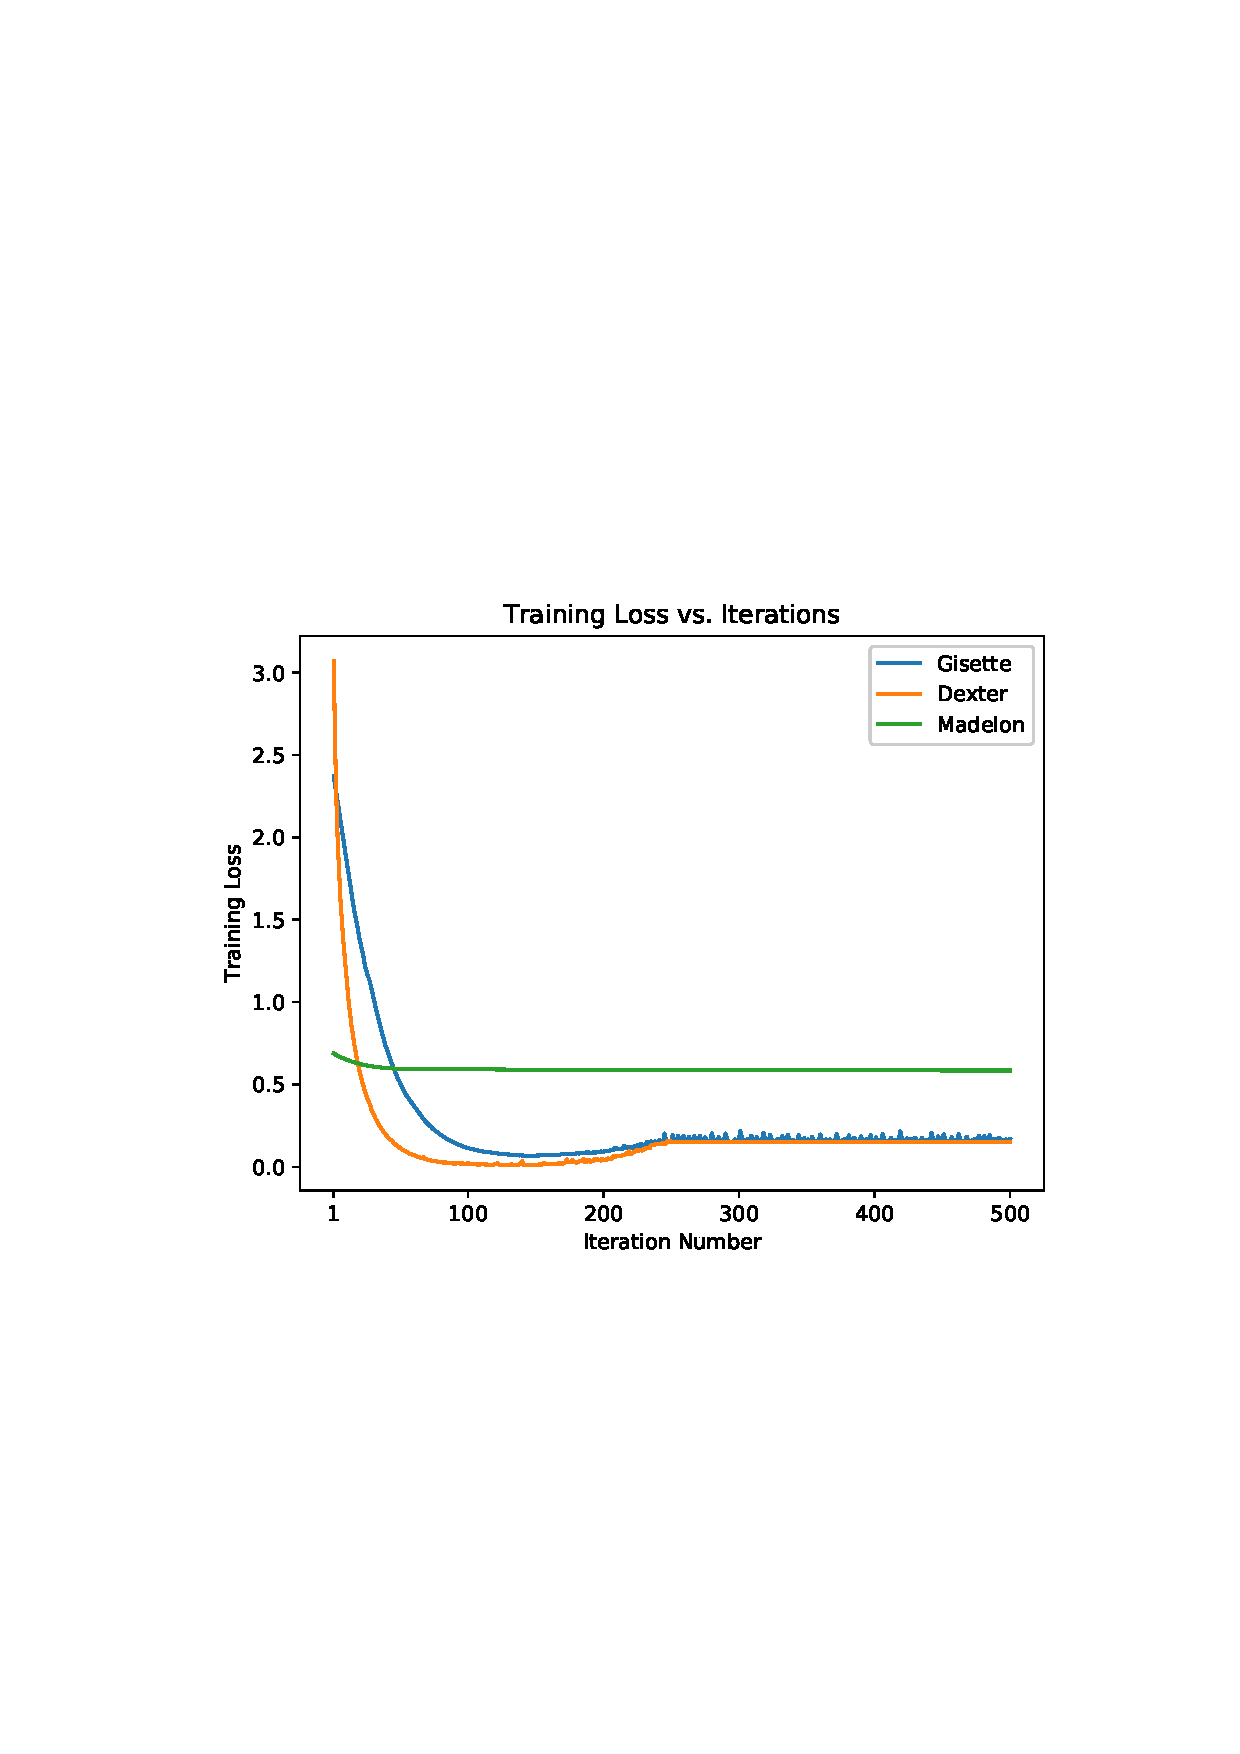
\includegraphics[scale=0.75]{./figures/graph.png}
\end{figure}

\end{document}
